%% Simplified vision for Ausarbeitungen
\documentclass[%
paper=a4,      % alle weiteren Papierformat einstellbar
fontsize=11pt, % Schriftgr��e (12pt, 11pt (Standard))
BCOR1cm,       % Bindekorrektur, bspw. 1 cm
DIV15,         % f�hrt die Satzspiegelberechnung neu aus s. scrguide 2.4
%twoside,       % Doppelseiten
headsepline,   %
headings=openright, % Kapitel nur rechts beginnen
%biblography=totoc, % Literaturverzeichnis einf�gen bibtotocnumbered: nummeriert
parskip=half,  % Europ�ischer Satz mit Abstand zwischen Abs�tzen
chapterprefix, % Kapitel anschreiben als Kapitel
headsepline,   % Linie nach Kopfzeile
titlepage,     %
numbers=noenddot,
%draft	       % zeigt �berlange Zeilen an
]{scrreprt}

\usepackage{pdfpages}       % Titelseite hat ein anderes Layout. Sie wird 
                            % separat erzeugt und hier eingef�gt
\usepackage[T1]{fontenc}
\usepackage[utf8]{inputenc}  % Zeichencodierung
\usepackage[ngerman, english]{babel} % Worttrennung nach neuer Rechtschreibung
%\usepackage[ngerman]{babel}
\usepackage{ellipsis}       % Leerraum um Auslassungspunkte
\usepackage{fixltx2e}       % Fehlerkorrektur Zeichens�tze
\usepackage{xspace}         % f�ge evtl. notwendiges Leerzeichen hinzu (\xspace)
\usepackage{textcomp}

%\usepackage{mathptmx}           % Times + passende Mathefonts
\usepackage{mathpazo}           % Palatino + passende Mathefonts
\usepackage[scaled=.92]{helvet} % skalierte Helvetica als \sfdefault
\usepackage{courier}            % Courier als \ttdefault
\usepackage{subcaption}

\usepackage{graphicx}    % Einbindung von Grafiken
\graphicspath{{Images/}} % Unterverzeichnis, in dem Grafiken abgelegt werden
\usepackage{listings}    % Listenausgabe externer Dateien

\usepackage{float}      % Paket zum Erweitern der Floatumgebungen
\usepackage[figuresright]{rotating}   % Rotieren von Objekten
%\usepackage{hvfloat}
\usepackage{array}      % Paket zum Erweitern der Tabelleneigenschaften
\usepackage{booktabs}   % Paket f�r sch�nere Tabellen

\usepackage{amsmath}    % erweiterte Mathematik-Umgebungen
\usepackage{amssymb}
\usepackage{url}



% Einstellungen f�r das Literaturverzeichnis
\usepackage[round]{natbib}
\setlength{\bibsep}{0.5\baselineskip}
\setlength{\bibhang}{1cm}
\bibliographystyle{agsm}

% Andere Schriftarten in Koma-Script
\setkomafont{sectioning}{\normalfont\bfseries}
\setkomafont{captionlabel}{\rmfamily\bfseries\small}
\setkomafont{caption}{\mdseries\itshape\small}
\setkomafont{pagehead}{\normalfont\itshape} % Kopfzeilenschrift
\setkomafont{descriptionlabel}{\normalfont\bfseries}

% Kopf und Fu�zeilen
\usepackage[automark]{scrlayer-scrpage}

% Hyperref
\usepackage{hyperref}

% Literaturverzeichnis-Stil
\bibliographystyle{plain}

% weitere Einstellungen
\tolerance=200               % �bervolle Zeile vermeiden
\emergencystretch=3em

\clubpenalty=10000           % 'Schusterjungen' und 'Hurenkinder' vermeiden
\widowpenalty=10000 
\displaywidowpenalty=10000

\parindent 0pt               % Einzug zu Absatzbeginn festlegen

\setcapindent{1em}           % Zeilenumbruch bei Bildbeschreibungen.

\setcounter{secnumdepth}{3}  % Strukturiertiefe bis subsubsection{} m�glich
\setcounter{tocdepth}{3}     % Dargestellte Strukturiertiefe im Inhaltsverzeichnis

% Korrekturversion mit 1.5-fachem Zeilenabstand im Hauptteil:
\newif\ifiscorrect
%\iscorrecttrue   % Korrekturversion
\iscorrectfalse % keine Korrekturversion

%% Eigene Definitionen:

% Einheiten:
\def\ut#1{\ensuremath{\,\mathrm{#1}}}

% Operatoren:
\def\grad{\ensuremath{\mathop{\mathrm{grad}}\nolimits}}
\def\transp#1{\ensuremath{{#1}^\mathsf{T}}}  % transpose
\def\const{\ensuremath{\mathop{\mathrm{const.}}\nolimits}}

% Formelzeichen:
\def\vec#1{\ensuremath{\mathbf{#1}}}
\def\matr#1{\ensuremath{\mathbf{#1}}}

% Hack, um ein zus�tzliches Leerzeichen nach \input zu entfernen:
\def\myinput#1{%
  \endlinechar=-1 % kein Zeilenabschlusszeichen
  \input #1\relax
  \endlinechar `\^^M % Zeilenabschluss = Zeilenvorschub
}



\begin{document}
\selectlanguage{ngerman}
\pagenumbering{Roman}
\pagestyle{plain}

%% Title

\includepdf[pages=1]{title}

%% Table of contents
\pagestyle{scrheadings}
\clearscrheadfoot            % Standardkram wegwerfen
\ohead[\pagemark]{\pagemark} % oben au�en Seitenzahl 
% Ausarbeitung简化版目录,只保留内容目录
\tableofcontents


% Pages number: roemisch
% Nmber in the text: arabic
\newcounter{roemisch}
\setcounter{roemisch}{\value{page}}
\pagenumbering{arabic}

\ifiscorrect\linespread{1.5}\selectfont % ???: 1 1/2 (f�r bessere Korrektur)
\else\fi

%% Chapters
% Kopfzeile: links Kapitel, rechts Sektion
\clearscrheadfoot            % Standardkram wegwerfen
\ohead[\pagemark]{\pagemark} % oben au�en Seitenzahl 
\ihead{\headmark}            % oben innen automatischer Abschnittsname
\automark[]{section}
\newpage
\chapter{}
\section{Einleitung}
Das amtliche Höhensystem in Deutschland basiert auf Normalhöhen $H_N$. Bezugsfläche dieses Höhensystems ist das Quasigeoid. In dieser Übung sind 30 Festpunkten mit Ellipsoidische Höhen gegeben, 20 davon haben bekannte Normalhöhen. Die übrige Normalhöhen sind angefragt. 
\newpage

\section{Aufgabe}
\subsection{a}
Höhenanomalie
\begin{equation*}
	\zeta = h - H_N
\end{equation*}
wobei
\begin{itemize}
	\item $h$: ellpsoidische Höhe
	\item $H_N$: Normalhöhe
\end{itemize}
Höhenanomalie von Punkten 1 bis 20: 
\begin{table}[ht] \centering
	\begin{tabular}{|l|l|}
		\hline
		Pkt.Nr & Höhenanomalie [\ut{m}] \\ \hline
		1     & 48,3548       \\ \hline
		2     & 48,3928       \\ \hline
		3     & 48,4118       \\ \hline
		4     & 48,4159       \\ \hline
		5     & 48,4290       \\ \hline
		6     & 48,3750       \\ \hline
		7     & 48,4098       \\ \hline
		8     & 48,4360       \\ \hline
		9     & 48,4360       \\ \hline
		10    & 48,4487       \\ \hline
	\end{tabular}
	\begin{tabular}{|l|l|}
		\hline
		Pkt.Nr & Höhenanomalie [\ut{m}] \\ \hline
		11    & 48,3946       \\ \hline
		12    & 48,4203       \\ \hline
		13    & 48,4420      \\ \hline
		14    & 48,4556       \\ \hline
		15    & 48,4695      \\ \hline
		16    & 48,4148       \\ \hline
		17    & 48,4483       \\ \hline
		18    & 48,4659       \\ \hline
		19    & 48,4762       \\ \hline
		20    & 48,4890       \\ \hline
	\end{tabular}
\end{table}
\\
Standardabweichung
\begin{equation*}
	\sigma_{\zeta} = \sqrt{(\sigma_h^2 + \sigma_{H_N}^2)} = 0,0051 \ut{m}
\end{equation*}
Graphische Darstellung:
\begin{figure*}[ht]\centering
	\begin{subfigure}{.8\textwidth}
		\centering
		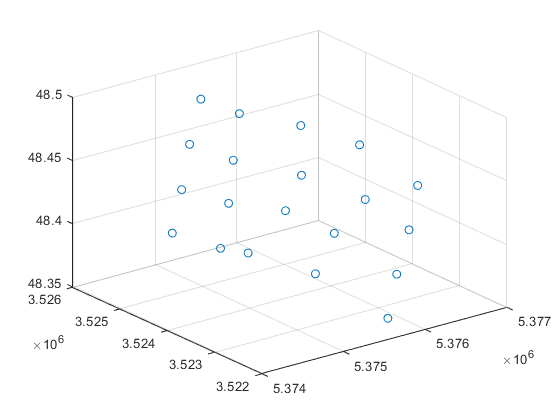
\includegraphics[width=.8\linewidth]{Images/Hoeheanomaliepunkt}  
		\caption{Höhenanomalie}
		\label{fig:sub-first}
	\end{subfigure}
\end{figure*}

\newpage
\subsection{b}
Der funktionale Modell:
\begin{gather*}
	\zeta_i = a_0 + a_1 \cdot y_i + a_2 \cdot x_i + a_3 \cdot y_i \cdot x_i + a_4 \cdot y_i^2 + a_5 \cdot x_i^2 \\
	\underbrace{\begin{bmatrix}
		\zeta_1 \\
		\zeta_2 \\
		\vdots \\
		\zeta_{19} \\
		\zeta_{20}
	\end{bmatrix}}_{\text{$l$}} = \underbrace{\begin{bmatrix}
		1 & y_1 & x_1 & y_1 \cdot x_1 & y_1^2 & x_1^2 \\
		1 & y_2 & x_2 & y_2 \cdot x_2 & y_2^2 & x_2^2 \\
		\vdots \\
		1 & y_{19} & x_{19} & y_{19} \cdot x_{19} & y_{19}^2 & x_{19}^2 \\
		1 & y_{20} & x_{20} & y_{20} \cdot x_{20} & y_{20}^2 & x_{20}^2 \\
	\end{bmatrix}}_{\text{$A$}} \cdot \underbrace{\begin{bmatrix}
		a_0 \\
		a_1 \\
		a_2 \\
		a_3 \\
		a_4 \\
		a_5
	\end{bmatrix}}_{\text{$x$}} \\
	\hat{x} = (A'A)^{-1}A'l = \begin{bmatrix}
		64990,1304 \\
		-0,0500 \\
		0,0086 \\
		1,3003 \cdot 10^{-8} \\
		-2,8173 \cdot 10^{-9} \\
		-5,0615 \cdot 10^{-9} \\
	\end{bmatrix}
\end{gather*}
\newpage
\subsection{c}
$n$ ist die Anzahl der übrigen Koeffizienten, $r = 20 - n$ \\
Kovarianzmatrix von alle Koeffizienten
\begin{gather*}
	\Sigma_{a} = \sigma_{\zeta}^2 \cdot (A'A)^{-1} \\
\end{gather*}
Standardabweichung von Koeffizienten:
\begin{equation*}
	\sigma_a = \sqrt{ diag(\Sigma_{a})}
\end{equation*}
Testgröße für eine Koeffizient
\begin{equation*}
	\frac{|a_i - 0|}{\sigma_{a_i}}
\end{equation*}
Quantil ist $t^t_{97,5,r}$ in t-Verteilung. \\
Testgröße in jeder Schleife: 
\begin{table}[ht] \centering
	\begin{tabular}{|l|l|l|l|l|l|l|l|}
		\hline
		& Quantil & $T_{a_0}$ & $T_{a_1}$  & $T_{a_2}$ & $T_{a_3}$ & $T_{a_4}$  & $T_{a_5}$  \\ \hline
		1 & 2,1448  & 1,2128e5  & -0,0814    & 0,0082    & 1,7880e-8 & -2,0830e-9 & -6,6258e-9 \\ \hline
		2 & 2,1314  & 4,9219e4  & -0,0279    &       & 1,0868e-8 & -4,3181e-9 & -3,5627e-9 \\ \hline
		3 & 2,1199  &       & -1,1886e-5 &      & 7,3875e-9 & -5,6267e-9 & -2,4217e-9 \\ \hline
	\end{tabular}
\end{table}
\newline
Koeffizienten in jeder Schleife:
\begin{table}[ht] \centering
	\begin{tabular}{|l|l|l|l|l|l|l|}
		\hline
		& $a_0$    & $a_1$      & $a_2$  & $a_3$     & $a_4$      & $a_5$      \\ \hline
		1 & $1,2128 \cdot 10^{-5}$ & -0,0814    & 0,0082 & $1,7880 \cdot 10^{-8}$ & $-2,0830 \cdot 10^{-9}$ & $-6,6258 \cdot 10^{-9}$ \\ \hline
		2 & 4,9219e4 & -0,0279    &     & $1,0868\cdot 10^{-8}$ & $-4,3181 \cdot 10^{-9}$ & $-3,5627 \cdot 10^{-9}$ \\ \hline
		3 &       & $-1,1886 \cdot 10^{-5}$ &     & $7,3875 \cdot 10^{-9}$ & $-5,6267 \cdot 10^{-9}$ & $-2,4217 \cdot 10^{-9}$ \\ \hline
	\end{tabular}
\end{table}
\begin{figure*}[ht]\centering
	\begin{subfigure}{.8\textwidth}
		\centering
		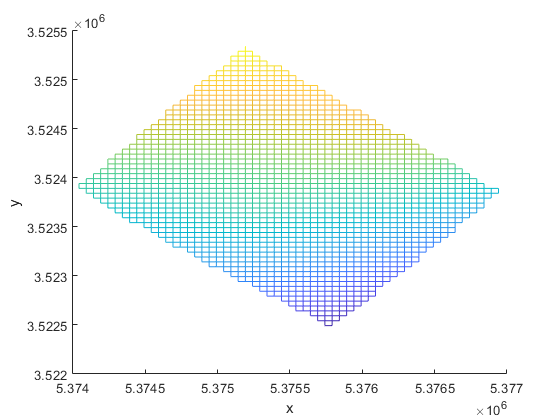
\includegraphics[width=.7\linewidth]{Images/Hoeheanomalie}  
		\caption{Höhenanomalie}
		\label{fig:sub-first}
	\end{subfigure}
\end{figure*}
\newpage
\subsection{d}
Wir haben jetzt das neue Flächenpolynom:
\begin{equation*}
	\zeta_i = a_1 \cdot y_i + a_3 \cdot y_i \cdot x_i + a_4 \cdot y_i^2 + a_5 \cdot x_i^2
\end{equation*}
Die Koordinaten der Neupunkten sind bekannt, damit darf man die Höhenanomalie berechnen.
\begin{table}[ht] \centering
	\begin{tabular}{|l|l|}
		\hline
		Pkt.Nr & Höhenanomalie [\ut{m}] \\ \hline
		21     & 48,4386       \\ \hline
		22     & 48,4397       \\ \hline
		23     & 48,4301       \\ \hline
		24     & 48,4303       \\ \hline
		25     & 48,4357       \\ \hline
		26     & 48,4465       \\ \hline
		27     & 48,4463       \\ \hline
		28     & 48,4413       \\ \hline
		29     & 48,4317       \\ \hline
		30    & 48,4199       \\ \hline
	\end{tabular}
\end{table}\\
Die ellipsoidesche Höhen sind bekannt, dann: 
\begin{table}[ht] \centering
	\begin{tabular}{|l|l|}
		\hline
		Pkt.Nr & Normalhöhe [\ut{m}] \\ \hline
		21     & 799,9974       \\ \hline
		22     & 791,3263       \\ \hline
		23     & 614,9569       \\ \hline
		24     & 570,9737      \\ \hline
		25     & 504,6443    \\ \hline
		26     & 495,1945       \\ \hline
		27     & 466,7147       \\ \hline
		28     & 441,3237       \\ \hline
		29     & 412,4763       \\ \hline
		30     & 376,8061      \\ \hline
	\end{tabular}
\end{table}
\newpage
\subsection{e}
Standardabweichung der Neupunktennormalhöhen sind durch Fehlerfortpflanzung bestimmbar. 
\begin{equation*}
	\Sigma_{neu} = F \cdot \Sigma_{ll} \cdot F'
\end{equation*} 
wobei:
\begin{gather*}
	F = \underbrace{\begin{bmatrix}
	1 & 0 & 0 & \cdots & 0 & 0 & y_{21} & y_{21} \cdot x_{21} & y_{21}^2 & x_{21}^2 \\
	0 & 1 & 0 & \cdots & 0 & 0 & y_{22} & y_{22} \cdot x_{22} & y_{22}^2 & x_{22}^2 \\
	0 & 0 & 1 & \cdots & 0 & 0 & y_{23} & y_{23} \cdot x_{23} & y_{23}^2 & x_{23}^2 \\
	\vdots & \vdots & \vdots & \cdots & \vdots & \vdots & \vdots & \vdots & \vdots & \vdots \\
	0 & 0 & 0 & \cdots & 1 & 0 & y_{29} & y_{29} \cdot x_{29} & y_{29}^2 & x_{29}^2 \\
	0 & 0 & 0 & \cdots & 0 & 1 & y_{30} & y_{30} \cdot x_{30} & y_{30}^2 & x_{30}^2 \\
	\end{bmatrix}}_{\text{$10 \times 14$}}
\end{gather*}
Die Standardabweichungen sind: 
\begin{table}[ht] \centering
	\begin{tabular}{|l|l|}
		\hline
		Pkt.Nr & Standardabweichung [\ut{mm}] \\ \hline
		21     & 5,4100       \\ \hline
		22     & 5,2923       \\ \hline
		23     & 5,2878       \\ \hline
		24     & 5,2675      \\ \hline
		25     & 5,2893    \\ \hline
		26     & 5,2625       \\ \hline
		27     & 5,4290       \\ \hline
		28     & 5,4597       \\ \hline
		29     & 5,4504       \\ \hline
		30     & 5,4347      \\ \hline
	\end{tabular}
\end{table}
\subsection{f}
Die Standardabweichung für $1 \ut{km}$ Doppelnivellement ist $0,4 \ut{mm}$.


\ifiscorrect\linespread{1.0}\selectfont% Zeilenabstand wieder auf 1 zur�ck
\else\fi

% Setze Numerierung wieder auf r�misch zur�ck und setzte von oben fort
% Wert ist demnach der von 'roemisch'
\newpage
\pagenumbering{Roman}
\setcounter{page}{\value{roemisch}}


\end{document}
